\documentclass{standalone}
%\usepackage{amsmath}\usepackage{lmodern}      % Matches the MathJax default (Latin Modern)
%\usepackage[T1]{fontenc}  % Ensures proper character encoding
\usepackage{tikz}
\usetikzlibrary{positioning, arrows.meta, calc}

% Document metadata (Safe to keep in preamble, standalone will skip them during crop)
\title{Chapter 03 — section 04 — diagram 06}
\author{0im}
\date{2026}

\begin{document}
    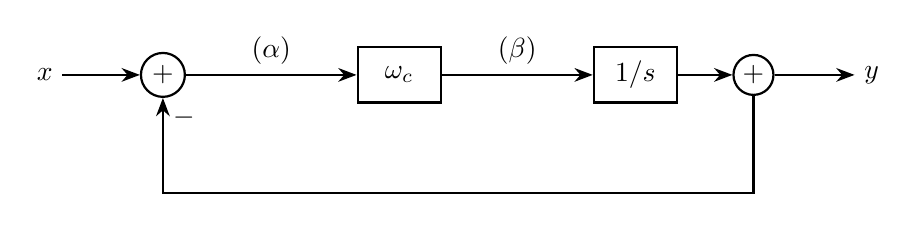
\begin{tikzpicture}
    [
        on grid, 
        node distance=1.5cm and 1.5cm, % Fixed: Added explicit cm units
        block/.style={draw, rectangle, minimum height=2em, minimum width=3em, thick},
        sum/.style={draw, circle, inner sep=2pt, thick},
        branch/.style={draw, circle, inner sep=1.5pt, thick}
    ]
        % =========================================================================
        % NODES
        % =========================================================================
        % --- Row 1 ---
        \node (x) {$x$};
        \node [sum, right=of x] (sum1) {$+$};
        \node [right=of sum1] (blank1) {};
        \node [block, right=of blank1] (cutoff1) {$\omega_c$};
        \node [right=of cutoff1] (blank2) {};
        \node [block, right=of blank2] (int1) {$1/s$};
        \node [branch, right=of int1] (branch1) {$+$};
        \node [right=of branch1] (y) {$y$};        
        % --- Row 2 ---
        \node [below=of sum1] (blank3) {};
        \node [below=of branch1] (blank4) {};
        
        % =========================================================================
        % PATHS
        % =========================================================================
        % --- HORIZONTAL ---
        %  Row 1
        \draw [-Stealth, thick] (x.east) -- (sum1.west);
        \draw [-Stealth, thick] (sum1.east) -- node [anchor=south] {$(\alpha)$} (cutoff1.west);
        \draw [-Stealth, thick] (cutoff1.east) -- node [anchor=south] {$(\beta)$} (int1.west);
        \draw [-Stealth, thick] (int1.east) -- (branch1.west);
        \draw [-Stealth, thick] (branch1.east) -- (y.west);
        % --- ANGLED ---
        \draw [-Stealth, thick]
            (branch1.south) -- (blank4.center) -- (blank3.center) -- (sum1.south)
            node [anchor=north west] {$-$};

    \end{tikzpicture}

\end{document}